% Cal Poly Thesis
% 
% based on UC Thesis format
%
% modified by Mark Barry 2/07.
%
%presented by Scott Winkleblack
%

\documentclass[12pt]{ucthesis}
\usepackage{ifpdf}

\newif\ifpdf
\ifx\pdfoutput\undefined
    \pdffalse % we are not running PDFLaTeX
\else
\pdfoutput=1 % we are running PDFLaTeX
\pdftrue \fi

\usepackage{url}
\usepackage{multicol}
\usepackage{cite}

\ifpdf
    \usepackage[pdftex]{graphicx}
    % Update title and author below...
    \usepackage[pdftex,plainpages=false,breaklinks=true,colorlinks=true,urlcolor=blue,citecolor=blue,
		linkcolor=blue,bookmarks=true,bookmarksopen=true,%
		bookmarksopenlevel=3,pdfstartview=FitV,
		pdfauthor={Kevin Schapansky},
		pdftitle={Jester: A Device Abstraction and Data Fusion API for Skeletal Tracking Sensors},
		pdfkeywords={thesis, masters, cal poly}]{hyperref}
    %Options with pdfstartview are FitV, FitB and FitH
    \pdfcompresslevel=1

\else
    \usepackage{graphicx}
\fi

\usepackage{hyperref}
\hypersetup{
	linktoc=all,
    colorlinks,
    citecolor=black,
    filecolor=black,
    linkcolor=black,
    urlcolor=black
}

\usepackage{titlesec}
% \titleformat{\chapter}[display]% OLD
%     {\normalfont\huge\bfseries}{\chaptertitlename\ \thechapter}{20pt}{\Huge}% OLD
% \titlespacing*{\chapter}{0pt}{50pt}{40pt}% OLD
\titleformat{\chapter}[display]% NEW
    {\normalfont\centering}{\chaptertitlename\ \thechapter}{12pt}{}% NEW
\titlespacing*{\chapter}{0pt}{30pt}{20pt}% NEW

%\titleformat{\section}[block]{first}{label}{12pt}

\titleformat{\section}{}{\thesection}{1em}{}
\titleformat{\subsection}{}{\thesubsection}{1em}{}
\titleformat{\subsubsection}{}{\thesubsubsection}{1em}{}
\titleformat{\paragraph}{}{\theparagraph}{1em}{}

\usepackage[font={}]{caption}

%\renewcommand{\cftchapleader}{\cftdotfill{\cftdotsep}} % for chapters
%\renewcommand{\cftsecleader}{\cftdotfill{\cftdotsep}} 

\usepackage{mathtools}
\DeclarePairedDelimiter{\ceil}{\lceil}{\rceil}
\usepackage{algorithmic}
\usepackage{amssymb}
\usepackage{amsmath}
\usepackage[letterpaper,papersize={8.5in,11in}]{geometry}
\usepackage[overload]{textcase}
\usepackage[toc,page]{appendix}

\usepackage{tabularx}
\usepackage{algorithm}
%\usepackage{algpseudocode}

\usepackage{enumitem}
\setlist{nolistsep}


\floatstyle{boxed}
\restylefloat{table}

%\bibliographystyle{abbrv}

\setlength{\parindent}{0.25in} \setlength{\parskip}{6pt}

\geometry{verbose,nohead,tmargin=1.25in,bmargin=1in,lmargin=1.5in,rmargin=1.3in}

\setcounter{tocdepth}{3}
\setcounter{secnumdepth}{3}


% Different font in captions (single-spaced, bold) ------------
%\newcommand{\captionfonts}{\small\bf\ssp}
\newcommand{\captionfonts}{}

\makeatletter  % Allow the use of @ in command names
\long\def\@makecaption#1#2{%
  \vskip\abovecaptionskip
  \sbox\@tempboxa{{\captionfonts #1: #2}}%
  \ifdim \wd\@tempboxa >\hsize
    {\captionfonts #1: #2\par}
  \else
    \hbox to\hsize{\hfil\box\@tempboxa\hfil}%
  \fi
  \vskip\belowcaptionskip}
\makeatother   % Cancel the effect of \makeatletter
% ---------------------------------------

\begin{document}

% Declarations for Front Matter

% Update fields below!
\title{Low-Cost Stereo Vision System for Autonomous Mobile Robots}
\author{Connor Citron}
\degreemonth{June} \degreeyear{2014} \degree{Master of Science}
\defensemonth{June} \defenseyear{2014}
\numberofmembers{3} \chair{Professor Chris Lupo, Ph.D.,\newline Department of Computer Science} \othermemberA{Professor Bruce Golden, Ph.D.,\newline Department of Dairy Science} \othermemberB{Professor John Seng, Ph.D.,\newline Department of Computer Science} \field{Computer Science} \campus{San Luis Obispo}
\copyrightyears{seven}

\maketitle

\begin{frontmatter}

% Custom made for Cal Poly (by Mark Barry, modified by Andrew Tsui).
\copyrightpage

% Custom made for Cal Poly (by Andrew Tsui).
\committeemembershippage

\begin{abstract}

Something, something, robots.
that


\end{abstract}

\begin{acknowledgements}

I would like to especially thank my parents and family for their love and support.

\end{acknowledgements}

\tableofcontents

\listoftables

\listoffigures

\end{frontmatter}

\pagestyle{plain}

\renewcommand{\baselinestretch}{1.66}

% ------------- Main chapters here --------------------

\chapter{Introduction}
\label{sec:intro}

Stereo vision uses two adjacent cameras to create a three dimensional image. This is similar to how human eyes work. A depth map can be created by comparing the offset of a pair of corresponding pixels of the two cameras. This depth map is a three dimensional representation of the real world. Mobile robots can use stereo vision to improve their awareness of their surroundings.

The point cloud made from the pixels of the depth map in combination with one of the actual images allows for object detection and object identification. As opposed to infrared laser scanning which can only be used indoors, stereo vision can be used anywhere there is adequate lighting. The data obtained from a stereo vision system can be used to map or recreate objects and places it has seen \cite{actStereoMap}.

Some of the earliest research of stereo vision was used with industrial robots \cite{industRobot}. In the 1980s, the challenge of industrial robots needing to avoid unexpected obstacles was addressed with stereo vision in order to detect those objects quickly and to determine how far the robot would need to adjust its course to prevent accidental collisions \cite{3DVision}.

As stereo vision systems become more essential for mobile robots, embedded stereo vision systems become more important. Embedded stereo vision systems allow for smaller robots to achieve the same capabilities as their larger counterparts \cite{xilinxSpartan3ABoard}.

One problem faced with stereo vision systems is the amount of information that needs to be processed to allow for real time operations, which can make the robot perform slowly \cite{nav}. Smaller image sizes will help speed up performance, but at the cost of the resolution of the objects in the images. 

Most of the image processing is independent of the rest of the image which allows for parallelization when processing each image. In the 1990s, research into using Field Programmable Gateway Arrays (FPGAs) with stereo vision began to gain momentum due to the parallelizability of FPGAs \cite{stereoFPGA}. In the 2000s and onward is when FPGAs became more practical for higher speeds and higher image resolutions for real time mobile robot applications \cite{fpga}.

Mobile robots such as autonomous quadrupeds are able to use stereo vision to navigate difficult terrain while avoiding obstacles in their path \cite{quadRobot}.

The stereo vision system module presented in this paper is used on a FPGA Atlys board~\cite{atlysBoard} and is shown to work with two different types of implementations of the Sum of the Absolute Differences (SAD) algorithm. 

Background information on stereo vision and the SAD algorithm used in stereo vision implementations in this paper can be found in Chapter 2. Related work is presented in Chapter 3. The implementation of the system used on the FPGA board is described in Chapter 4. Experiments and results are presented in Chapter 5. Finally, the conclusion and future work are in Chapter 9 and Chapter 10, respectively.

%%\include{chapters/Motivation}

\chapter{Background}
\label{bckgrnd}

This chapter presents some general information on stereo vision that be useful for understanding the decision that were made in developing this stereo vision system.

\section{Computer Stereo Vision}

Computer vision is concerned with using computers to understand and use information that is within visual images ~\cite{computerVision}. There are many different types of computer vision, which range from using one image to multiple images to obtain information. One image is not enough to determine the three dimensional properties of the objects within the image.

Stereo vision uses multiple images of the same scene in order to construct a three dimensional representation of the objects in the images ~\cite{stereoVision}. Comparing multiple images together for their similarities and differences allows for the depth to be obtained.

Binocular stereo ~\cite{binocularStereo} involves comparing a pair of images. These images are normally acquired simultaneously from a scene. By searching for corresponding pairs of pixels between the two images, depth information can be determined ~\cite{binocularStereo}. Pixel based comparisons can require substantial amount of computational power and time. Certain assumptions are made because of the computational resources required. Camera calibration and epipolar lines [cite 14-14 and define better] are common assumptions. For example, two images of the same scene are 640 x 480 pixels in size. Each image therefore contains 307,200 pixels, which is over 600,000 pixels between the two images for one frame. For a real-time application, say 30 frames per second for example, that becomes over 18 million pixels between the two images that would need to be processed every second.

Computational requirements for real-time applications can be reduced in several ways. First, by lowering the number of pixels in the images reduces the number of pixel comparison per second. Images at a size of 320 x 240 pixels would require a quarter of the number of computations at the cost of losing some amount of detail in the images. Also, reducing the number of frames per second will decrease the amount of computing needed. Going much below 30 frames per second is noticeable to a person and can be annoying to observe a slow frame rate. A robot on the other hand, depending on its task and how fast its moving, might only need a few frames per second in order to function within a desired range. So image resolution could be more important than frames per second for a robot if details are more important than speed.

Figure~\ref{fig:sv_diagram} below represents a simplified illustration of binocular stereo vision. The two cameras are held at a known fixed distance from each other and are used to triangulate different the distance of objects in the images they create. The points U\textsubscript{L} and U\textsubscript{R} in the left and right images, respectively, are 2D represents the point P that is in 3D space. By comparing the offset of between U\textsubscript{L} and U\textsubscript{R} in the two images, it is possible to obtain the distance of point P away from the cameras ~\cite{stereoVisionDiagram}.

\begin{figure}
	\begin{center}
		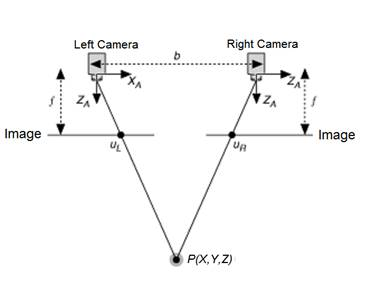
\includegraphics{figures/stereoVisionDiagram.jpg}
		\captionfonts
		\caption{Simplified binocular stereo vision system ~\cite{stereoVisionDiagram}.}
		\label{fig:sv_diagram}
	\end{center}
\end{figure}

The closer an object is to the stereo vision system, the greater the offset of corresponding pixels will be. If an object is too close to the system, it is possible for one camera to see part of an object that the other camera cannot. The farther an object is away from the stereo vision system, the smaller the offset of corresponding pixels will be. If an object is far enough away, it is possible for an object to be in almost the exact same location in both images. You can show this to yourself by holding a finger up close to your face, close one eye, and then alternate between which eye is open and which eye is closed. Your finger should appear to move a noticeable amount. Next, hold your finger as far away from you as you can and again alternate between which eye is open and which is closed. You should notice that your finger appears to move significantly less than it did when your finger was close to your face. That is how stereo vision works. The distance of an object is inversely proportional to the amount of offset between the two images.

\subsection{Parallelism in Stereo Vision}

Processing images for stereo vision allows for a high degree of parallelism. Locating the corresponding position of a pair of pixels is independent of finding another corresponding pair of pixels. This independent nature allows for the ability to process different parts of the same images at the same time, if there is hardware to support it.

Field Programmable Gate Arrays (FPGAs) allow for parallel processing to be implemented of the images. In section \textbf{(Implementation)} the amount of parallel processing used for the modular stereo vision system presented in this paper is discussed. 

\section{Stereo Vision Algorithms}

Stereo vision algorithms can be placed into one of three different categories: pixel-based methods, area-based methods, and feature-based methods ~\cite{similarAlgorithms}. Pixel-based methods utilize pixel by pixel comparisons. They can produce dense disparity \textbf{(define!)} maps, but at the cost of higher computation complexity and higher noise sensitivity ~\cite{similarAlgorithms}. Area-based methods utilize block by block comparisons. They can also produce dense disparity maps and are less sensitive to noise, however, accuracy tends to be low in areas that are not smooth ~\cite{similarAlgorithms}. Feature-based methods utilize features, such as edges and lines for comparisons. They cannot produce dense disparity maps, but have a lower computational complexity and are insensitive to noise ~\cite{similarAlgorithms}. 

There are a lot of stereo vision algorithms out there ~\cite{taxonomy}. In the taxonomy of ~\cite{taxonomy}, 20 different stereo vision algorithms were compared against each other using various reference images. Many algorithms are based on either the sum of absolute differences (SAD) or correlation algorithms ~\cite{alteraStratixIVPaper}.

An algorithm that is similar to SAD is Sum of the Square Differences (SSD). Both of these algorithms produce similar results and contain around the same amount of error ~\cite{similarAlgorithms}. SAD was chosen over the other algorithms to implement because it is simpler to implement in hardware. SSD requires squaring the difference between corresponding pixels and summing it up. Since squaring a number is the number multiplied by itself, the number will be added to itself that many times to produce the squared value. This is a lot more over head, and more hardware, than just taking the absolute difference of the difference of each corresponding pair.

\subsection{Sum of the Absolute Differences Algorithm}

SAD is a pixel-based matching method ~\cite{alteraStratixIVPaper}. Stereo vision uses this algorithm to compare a group of pixels called a window from one picture with a window in another picture. The SAD algorithm, shown in Equation~\ref{eq:sadAlg1} ~\cite{alteraStratixIVPaper}, takes the absolute difference between each pair of corresponding pixels and sums all of those values together to create a SAD value. One SAD value by itself does not give any useful information about those two corresponding windows. Several SAD values will be calculated from different candidate windows for each reference window. Out of the all the SAD values calculated for the reference window, the SAD value with the smallest value (all of them are positive because of the absolute part in the equation) is determined to contain the matching pixel. Figure~\ref{fig:sad_corr} shows for one reference window, there are several candidate windows used. The line that the candidate windows move across are called epipolar lines. 

\begin{equation}
	\sum\limits_{(i,j)\in W}\left| I_{1}(i,j)-I_{2}(x+i,y+j) \right|
	\label{eq:sadAlg1}
\end{equation}

\begin{figure}
\begin{center}
	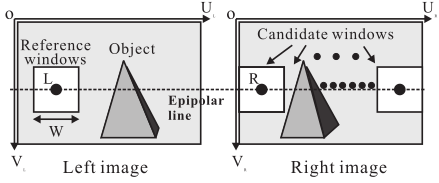
\includegraphics{figures/sadCorrespondingWindows.png}
	\captionfonts
	\caption{Searching for corresponding points between the two images ~\cite{sadParallel}.}
	\label{fig:sad_corr}
\end{center}
\end{figure}

In stereo vision, epipolar lines are created from the two cameras capturing images from the same scene. Figure~\ref{fig:epipolar} show the epipolar line that point X must be on in the corresponding images. This is useful because if the epipolar lines are known for both images, then it is possible to know the line that two corresponding points are on. It reduces the problem of finding the the same two points from a 2D area to a 1D line. Now, if the epipolar lines in both images are horizontal as they are in Fig.~\ref{fig:sad_corr} as opposed to them being at a diagonal as they are in Fig.~\ref{fig:epipolar} then Eq.~\ref{eq:sadAlg1} reduces to Equation ~\ref{eq:sadAlg2}. For cameras that are not perfectly aligned, rectification is often used in order to align epipolar lines between images ~\cite{rectification}. However, many stereo vision algorithms will assume that the epipolar lines are rectified to simplify the overall processing required.

\begin{figure}
\begin{center}
	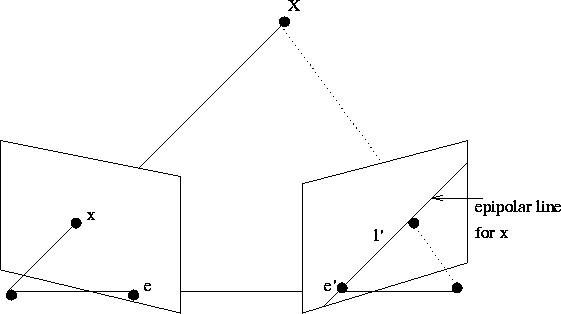
\includegraphics[height=50mm]{figures/epipolar.png}
	\captionfonts
	\caption{The epipolar line that point X is on for both images ~\cite{epipolar}.}
	\label{fig:epipolar}
\end{center}
\end{figure}

\begin{equation}
	\sum\limits_{(i,j)\in W}\left| I_{1}(i,j)-I_{2}(x+i,j) \right|
	\label{eq:sadAlg2}
\end{equation}

The disparity is the amount of offset between two corresponding pixels. The disparity range is the range that the candidate window will move through the image and is represented by the value 'x' in Eq.~\ref{eq:sadAlg2}. It corresponds to the amount of SAD values that will be calculated. Figure~\ref{fig:sadGraphs} shows two types of SAD search methods. Fig.~\ref{fig:globalSAD} selects the overall SAD value with the lowest value to be the matching pixel. However, Fig.~\ref{fig:localSAD} limits the search region to a specific area. This helps to avoid issues of similar looking areas that are not near the reference window from being falsely identified as matching. The downside to this is that if an object gets too close, meaning it would have high disparity values, and if the search region is not large enough, then the objects distance will be miss classified. It is important to determine a window size and a search region that are not too small and are not too big.

\begin{figure}
\begin{center}
	\begin{subfigure}{0.4\textwidth}
		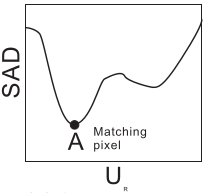
\includegraphics[width=\textwidth]{figures/sadGlobalGraph.png}
		\caption{Global SAD search}
		\label{fig:globalSAD}
	\end{subfigure}
	\begin{subfigure}{0.4\textwidth}
		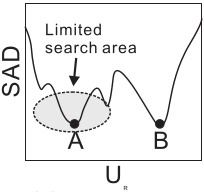
\includegraphics[width=\textwidth]{figures/sadLocalGraph.png}
		\caption{Local SAD search}
		\label{fig:localSAD}
	\end{subfigure}
	\captionfonts
	\caption{The SAD between a reference window and several candidate windows ~\cite{sadParallel}.}
	\label{fig:sadGraphs}
\end{center}
\end{figure}

For example, Figure ~\ref{fig:windows} shows a template window (Figure~\ref{fig:template}) from one image and the search area (Figure~\ref{fig:search}) in the other window. The disparity range is three, or zero to two. There are three 3x3 windows within the search region in Fig.~\ref{fig:search}. From left to right the three search windows have the center pixel as 4, 6, and 5, respectively. 

Comparing corresponding pixels in the template window with the first search window (let's call it S0) gives the absolute differences for all nine pixels going from left to right and top to bottom of 8, 1, 1, 2, 1, 0, 1, 2, and 2. So the SAD value for S0 of 18 is obtained by adding up all nine of those values. The SAD value for the second search window (S1) is 6 and the last search window (S2) is 13. The template window has the smallest difference between S1, which means that the center pixel in S1 is determined to be the corresponding pixel for the center pixel in the template window. 

The disparity value is 1 (how far the matching search window was shifted to the left). The disparity value is used to create a disparity map. Each disparity value in the disparity map is at the same relative location that the center pixel of its corresponding template window is located.

\begin{figure}
\begin{center}
	\begin{subfigure}{0.3\textwidth}
		\begin{center}				
			\begin{tabular}{|l|c|r|}
				\hline
				1 & 2 & 3 \\\hline
	  			4 & 5 & 6 \\\hline
		    	7 & 8 & 9 \\
		    	\hline
			\end{tabular}
		\end{center}
		\caption{Template Window}
		\label{fig:template}
	\end{subfigure}
	\begin{subfigure}{0.3\textwidth}
		\begin{center}		
			\begin{tabular}{|l|c|c|c|r|}
				\hline
				9 & 1 & 2 & 4 & 5 \\\hline
		  		2 & 4 & 6 & 5 & 3 \\\hline
		    	8 & 6 & 7 & 8 & 7 \\
		    	\hline
			\end{tabular}
		\end{center}
		\caption{Search Region}
		\label{fig:search}
	\end{subfigure}
	\captionfonts
	\caption{Template (reference) window and search (candidate) window.}
	\label{fig:windows}
\end{center}
\end{figure}










%\begin{figure}
%\begin{center}
%	\begin{subfigure}{0.3\textwidth}
%		\begin{center}				
%			\begin{tabular}{|l|c|r|}
%				\hline
%				1 & 2 & 3 \\\hline
%	  			4 & 5 & 6 \\\hline
%		    	7 & 8 & 9 \\
%		    	\hline
%			\end{tabular}
%		\end{center}
%		\caption{Template Window}
%		\label{fig:template}
%	\end{subfigure}
%	\begin{subfigure}{0.3\textwidth}
%		\begin{center}		
%			\begin{tabular}{|l|c|r|}
%				\hline
%				1 & 2 & 3 \\\hline
%		  		4 & 5 & 6 \\\hline
%		    	7 & 8 & 9 \\
%		    	\hline
%			\end{tabular}
%		\end{center}
%		\caption{Search Window}
%		\label{fig:search}
%	\end{subfigure}
%	\captionfonts
%	\caption{Template (reference) window and search (candidate) window.}
%	\label{fig:windows}
%\end{center}
%\end{figure}







\chapter{Related Work}

There are several different ways to implement a stereo vision system. Many stereo vision systems are implemented on field-programmable gate arrays (FPGAs). FPGAs allow for parallelization when processing images. Systems that use FPGAs generally can achieve a high frames per second with a decent or good image quality, but most of these systems are expensive. 

FPGA Design and Implementation of a Real-Time Stereo Vision System~\cite{alteraStratixIVPaper} uses an Altera Stratix IV GX DE4 FPGA board to process the right and left images that come from the cameras that were attached to it.~\cite{alteraStratixIVPaper} uses the Sum of Absolute Differences (SAD) algorithm to compute distances. This system allows for real time speeds, up to 15 frames per second at an image resolution of 1280x1024. However, the Altera Stratix IV GX DE4 FPGA board costs over \$4,000~\cite{alteraStratixIVBoard}, which makes the system impractical for non-high budget projects.

Improved Real-time Correlation-based FPGA Stereo Vision System~\cite{xilinxVirtex5Paper} uses a Xilinx Virtex-5 board to process images.~\cite{xilinxVirtex5Paper} uses a correlation-based algorithm, which is based on the Census Transform, to obtain the depth in images. The algorithm is fast, but there are some inherent weaknesses to it. This system can run at 70 frames per second for images at a resolution of 512x512. Unfortunately, the Xilinx Virtex-5 board costs more than \$1,000~\cite{xilinxVirtex5Board}, which is still expensive.

Low-Cost Stereo Vision on an FPGA~\cite{lowCost1000} uses a Xilinx Spartan-3 XC3S2000 board.~\cite{lowCost1000} uses the Census Transform algorithm for image processing. This allows images with a resolution of 320x240 to be processed at 150 frames per second. The total hardware for the low-cost prototype used in~\cite{lowCost1000} costs just over \$1,000, which is a bit too pricy for a lot of projects.

An Embedded Stereo Vision Module For Industrial Vehicles Automation~\cite{xilinxSpartan3APaper} uses a Xilinx Spartan-3A-DSP FGPA board.~\cite{xilinxSpartan3APaper} uses an Extended Kalman Filter (EKF) based visual simultaneous localization and mapping (SLAM) algorithm. The accuracy of this system directly varied with speed and distance of detected object. The Xilinx Spartan-3A-DSP FGPA board is  around \$600,~\cite{xilinxSpartan3ABoard} which is less costly than the others presented so far.

Several commercial stereo vision systems exist presently~\cite{xilinxSpartan3APaper}. Most of them are quite capable of producing good quality depth maps of their surroundings. However, the cost of these products can be relatively expensive, especially from a club or hobbyist standpoint. The Bumblebee2~\cite{bumblebee} from Point Gray is able to produce disparity maps at a rate of 48 frames per second for an image size of 640x480, but it costs somewhere around \$1,000 or so. Having been involved with the Cal Poly Robotics Club for 6 years and seen the budgets each project in the club usually gets, \$1,000 would be most of a project's budget for the year. That kind of money could be better spent elsewhere on the project.

During the course of this thesis, a stereo vision surveillance application paper~\cite{surveillance} was published that used the Digilent Atlys board~\cite{atlysBoard}. A stereo camera module, VmodCAM~\cite{vmodcam}, can be purchased with the Atlys board and was also used. The Atlys board is relatively cheap, at least by the standards presented thus far, at \$230 for academic use. With the VmodCam included, the price goes around \$350, which is still significantly cheaper than the other FPGA boards presented from other papers. The costs and capacity of the board are why the Atlys board was selected for use in this thesis (the selection was independent of the surveillance paper). The surveillance paper used the AD Census Transform to calculate distance. Their board output the disparity map data over HDMI to a monitor. The output image is rather noisy, but it is very easy for a human to understand what is in the image, which is its intended purpose.

%\include{chapters/Methodology}
%
%\include{chapters/Algorithm}

\chapter{Implementation}
\label{sec:impl}

This chapter presents the implementation and architecture of stereo vision system presented in this paper.

\section{Architecture Overview}

The stereo vision module in this paper is composed of three main parts: SAD, minimum comparators, and a wrapper, which goes around the previous two that takes in image data and outputs disparity values.

The code for the following sections is located on github under:
\\\path{https://github.com/cccitron/mastersThesis}.

\subsection{Sum of the Absolute Differences Architecture}

Two versions of the SAD algorithm have been implemented in this paper. The first uses a 9x9 window and the other one uses a 7x7 window. Figure~\ref{fig:sadAlg_rtl} shows the top level entity of the SAD implementation used. Both versions have a clocked input (clk\_I) and a one bit data input (data\_I) to notify the algorithm to begin calculating the SAD value. The template\_window\_I and search\_window\_I between the two versions differ in the sense that the number of bytes, 49 or 81, sent to the sadAlgorithm entity are different. The data\_O signal notifies when the calculation is complete and that it is ready for the next set of input. The calculated SAD value is sent out of the entity through sad\_O.

There is a slight variation between the standard SAD algorithm and how it is implemented in this stereo vision system. Instead of subtracting two pixel values and then taking the absolute difference between them, the implementation in this paper finds which corresponding pixel has a greater value and then sends the two pixels to the subtracter based on that. See Appendix~\ref{sec:appdxA} and Appendix~\ref{sec:appdxB} for the code used. The subtracter then takes the greater value and subtracts from it the lesser value and returns the difference, sub. The value sub will always be greater than or equal to zero, which is equal to the absolute difference of the two corresponding pixels. This process was implemented to reduce the complexity by not needing signed values and allowed for the number of bytes used for logic in the algorithm to be reduced since the values no longer need additional bits to account for the signed portion of negative values.

\begin{figure}[h]
	\begin{center}
		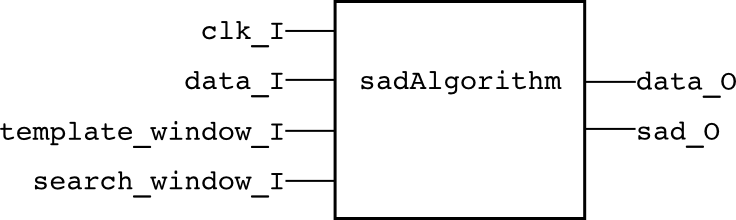
\includegraphics[width=100mm]{figures/sadAlgorithm_rtl.png}
		\captionfonts
		\caption{The top level SAD algorithm implementation.}
		\label{fig:sadAlg_rtl}
	\end{center}
\end{figure}

\subsubsection{State Diagram}

Inside the sadAlgorithm entity from Fig.~\ref{fig:sadAlg_rtl}, the state machine from Figure~\ref{fig:stateMachine} controls the SAD algorithm. The state machine begins at state SO and initializes all the values used in it to 0. It then proceeds to S1 where the state machine remains on standby until data\_I becomes `1'. In S2, the counter starts at 0, the subtraction between corresponding pixel values begins, and on the next clock cycle, the state will be S3. While in S3, the counter is incremented by 1 every clock cycle. S3 is where the SAD algorithm is performed. After the counter is equal to windowSize (7 for the 7x7 and 81 for the 9x9, see Section~\ref{sec:9x9window} and Section~\ref{sec:7x7window} for details) the SAD calculation is complete. The state machine sets data\_O to `1' to notify the SAD wrapper that the calculation is complete and the state moves to S1 and waits for the next set of input.

\begin{figure}[h]
	\begin{center}
		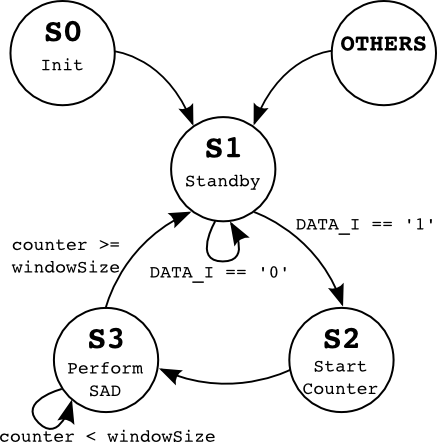
\includegraphics[width=100mm]{figures/stateMachine.png}
		\captionfonts
		\caption{The state machine for implementing the SAD algorithm.}
		\label{fig:stateMachine}
	\end{center}
\end{figure}

\subsubsection{9x9 Window}
\label{sec:9x9window}

The 9x9 window implementation operated with 4 pixels processed in parallel. Every pixel has 16 SAD operations processed in parallel. There are 64 SAD operations total occurring in parallel for the 4 pixels. However, each SAD calculation has a higher degree of serialization than the 7x7 window implementation in order to reduce space to fit on the Atlys board~\cite{atlysBoard}. Figure~\ref{fig:sadAlg9x9} shows a simplified version of this process. Each clock cycle, for 81 cycles, the difference between corresponding pixels is calculated. Beginning one clock cycle after the differences start to be calculated the difference, sub, sum\_out is added to itself and sub. This process also occurs 81 times, one addition each clock cycle. The state machine in Fig.~\ref{fig:stateMachine} stops the calculation for sum\_out after the full SAD value has been summed up.

\begin{figure}[h]
	\begin{center}
		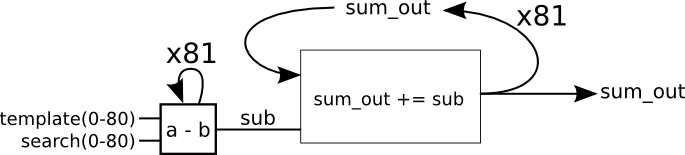
\includegraphics[width=120mm]{figures/sadAlgorithm9x9.png}
		\captionfonts
		\caption{Architecture overview of the SAD algorithm with the 9x9 window implementation.}
		\label{fig:sadAlg9x9}
	\end{center}
\end{figure}

Figure~\ref{fig:sadPipe9x9} illustrates the pipeline used in a SAD calculation in a SAD calculation for the 9x9 window version. It takes 81 clock cycles to take all of the differences between all 81 pairs of pixel values. After the first difference is calculated, the differences can then begin to be summed up. The summing also takes 81 clock cycles and ends one cycle after the last difference is calculated. This results in it taking 82 clock cycles.

\begin{figure}[h]
	\begin{center}
		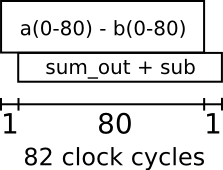
\includegraphics[width=50mm]{figures/sadPipeline9x9.png}
		\captionfonts
		\caption{Pipeline architecture of the SAD algorithm with the 9x9 window implementation.}
		\label{fig:sadPipe9x9}
	\end{center}
\end{figure}

The code for the 9x9 window implementation can be found on github:
\\\path{https://github.com/cccitron/mastersThesis/tree/master/makestuff/libs/libfpgalink-20120621/hdl/fx2/vhdl/sad_simple_reg_9x9}

\subsubsection{7x7 Window}
\label{sec:7x7window}

The 7x7 window implementation operated with 2 pixels processed in parallel. Each pixel has 16 SAD operations processed in parallel. There are only 32 SAD operations occurring in parallel, as opposed to 64 that were performed in parallel in Sec.~\ref{sec:9x9window}. The 7x7 window size has 32 pixels less than the 9x9 version for each window in every SAD calculation. The process was able to utilize a higher degree of parallelization. The increased parallelism takes up more space on the board than the serial version from Sec.~\ref{sec:9x9window}. Figure~\ref{fig:sadAlg7x7} shows a simplified version of this process. Each clock cycle during 7 cycles, the difference, sub, between corresponding pixels is calculated. One clock cycle after the differences begin to be calculated, sum\_out is added to itself and the value sub. This process also occurs 7 times, one set of addition each clock cycle. The state machine in Fig.~\ref{fig:stateMachine} stops the calculation for sum\_out after the full SAD value has been summed up.

The main difference between this implementation and the 9x9 window implementation from Sec.~\ref{sec:9x9window} is that the difference between corresponding pixels is parallelized to calculate 7 absolute differences at once. The dotted box in Fig.~\ref{fig:sadAlg7x7} represents all 7 of the subtraction calculations occurring 7 times in the SAD calculation. Instead of requiring 49 clock cycles to calculate all the differences, it only takes 7 clock cycles. All 7 of the differences that were calculated are added to sum\_out each clock cycle.

\begin{figure}[h]
	\begin{center}
		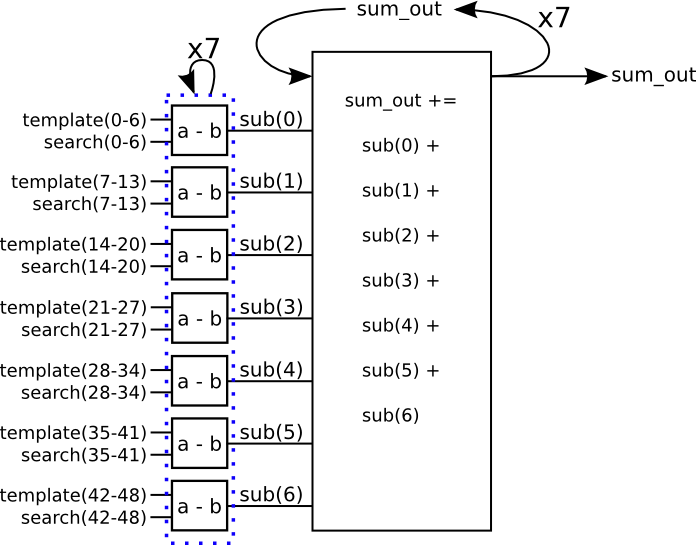
\includegraphics[width=130mm]{figures/sadAlgorithm7x7.png}
		\captionfonts
		\caption{Architecture overview of the SAD algorithm with the 7x7 window implementation.}
		\label{fig:sadAlg7x7}
	\end{center}
\end{figure}

Figure~\ref{fig:sadPipe7x7} shows the pipeline used for the 7x7 window version. It takes 7 clock cycles to take all of the differences between all 49 pairs of pixel values. After the first set of differences is calculated, the differences can begin to be summed up. The summing also takes 7 clock cycles and ends one cycle after the last difference is calculated. This results in a total of 8 clock cycles.

\begin{figure}[h]
	\begin{center}
		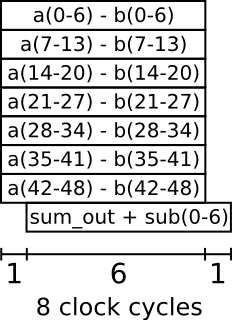
\includegraphics[width=50mm]{figures/sadPipeline7x7.png}
		\captionfonts
		\caption{Pipeline architecture of the SAD algorithm with the 7x7 window implementation.}
		\label{fig:sadPipe7x7}
	\end{center}
\end{figure}

The code for the 7x7 window implementation can be found on github:
\\\path{https://github.com/cccitron/mastersThesis/tree/master/makestuff/libs/libfpgalink-20120621/hdl/fx2/vhdl/sad_parallel_7x7}

\subsection{Minimum Comparator Architecture}

The purpose of the minimum comparator is to find the lowest value of two input values and output the lowest value. The top level implementation of the minimum comparator is shown in Figure~\ref{fig:minComp_rtl}. The process is synchronous, noted by the clock clk\_I. The index, pos0\_I and pos1\_I, of the SAD values sad0\_I and sad1\_I, respectively, ranges from 0 to 15, which gives a disparity range of 16. 

Appendix~\ref{sec:appdxC} shows the code for the minimum comparator. If sad1 is less than sad0, then sad1 and its index, pos1, are returned, otherwise sad0 and pos0 are returned. Using a less than comparison is supposed to take up less hardware than a greater than or equal to comparison~\cite{lessThan}. This is useful because 15 minimum comparators (see Figure~\ref{fig:minComp}) are used for each pixel that is processed in parallel. So 30 minimum comparators are used for the 7x7 window implementation and 60 minimum comparators are used for the 9x9 window implementation. Constructing the minimum comparator in this way accounts for cases where 2 SAD values are equal to each other. The SAD value with the lower index is always assigned to the sad0\_I input and the higher indexed SAD value goes to the sad1\_I input. Therefore, if 2 values are equal, the SAD value with a lower index, and a lower disparity, will be returned. This assumes if two SAD values are equal to each other the value with the index closer to 0 is more likely to be correct.

\begin{figure}[h]
	\begin{center}
		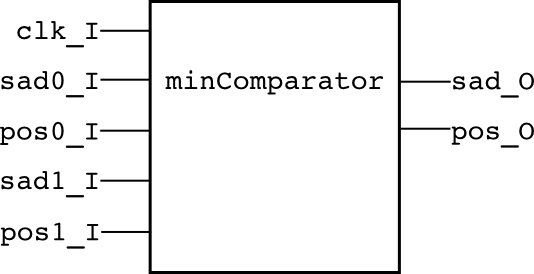
\includegraphics[width=90mm]{figures/minComparator_rtl.png}
		\captionfonts
		\caption{The top level minimum comparator implementation.}
		\label{fig:minComp_rtl}
	\end{center}
\end{figure}

When multiple minimum comparators are put together to create a tree, as shown in Fig.~\ref{fig:minComp}, it is possible to quickly determine which SAD value is the lowest. This process is used to find the index of the lowest SAD value out of the 16 SAD values calculated for each pixel. A normal serial comparison of 16 values would take 15 comparisons, or 15 clock cycles, if one comparison occurred each clock cycle. By having 15 comparators, the number of SAD values needed to be compared can be reduced by half each clock cycle. Using a tree of comparators drops the comparison time from 15 clock cycles to only 4 clock cycles. It is almost a 4 times speed up.

\begin{figure}[h]
	\begin{center}
		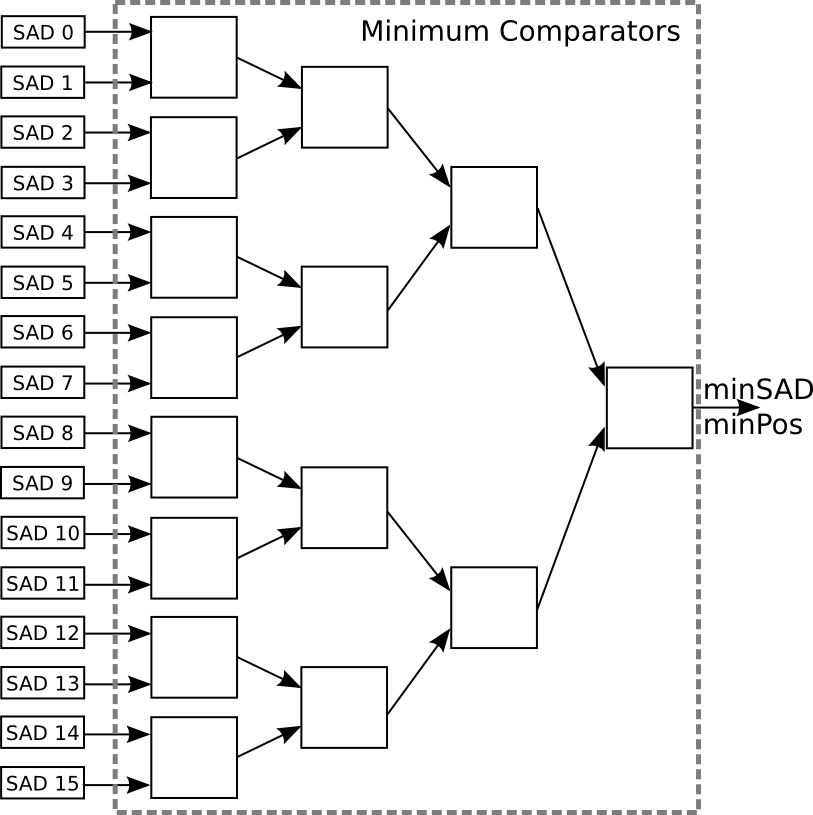
\includegraphics[width=150mm]{figures/minComparator.png}
		\captionfonts
		\caption{The minimum comparator tree designed to quickly find the minimum value and corresponding index out of the 16 SAD values that are calculated for one pixel.}
		\label{fig:minComp}
	\end{center}
\end{figure}

\subsection{SAD Wrapper}

The SAD wrapper is the entity that encompasses the SAD algorithms and minimum comparators. The wrapper gets a clock signal through clk\_I and a reset signal through rst\_I. It receives the template image data through templ\_I and receives the search image data through search\_I. The write\_t\_I and write\_s\_I notify the wrapper when new data is actively being sent for the template and search images, respectively. It is designed to allow data from both images to be sent to the wrapper in parallel or serially. The h2fReady\_I and f2hReady\_I are used to communicate when data is being sent to or from the host, the computer, from or to the FPGA. The sw\_I allows the 8 switches on Atlys board to be connected to data that is within the wrapper to be displayed on the 8 LEDs, led\_O. The outputs templ\_O for template image region, search\_O for search image region, sad\_O for the SAD values calculated from the current template and search image regions, and disp\_O that were found from the SAD values are outputted so they can be read, if desired. In the current implementations, templ\_O, search\_O, and sad\_O are used for debugging purposes only while disp\_O is used to create the depth map. See Section~\ref{sec:fpgalink} for how the data is transferred to the computer.

\begin{figure}[h]
	\begin{center}
		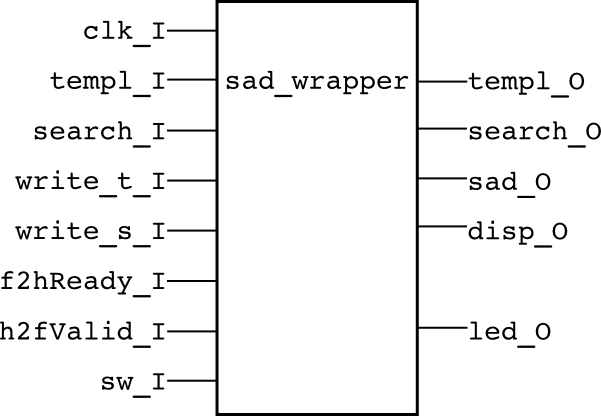
\includegraphics[width=90mm]{figures/sad_wrapper_rtl.png}
		\captionfonts
		\caption{The SAD wrapper that encompasses the SAD algorithm and minimum comparator. It interacts with the top level.}
		\label{fig:sadWrapper_rtl}
	\end{center}
\end{figure}

\subsection{Top Level}

The implementation of the SAD wrapper and its internal entities were designed to be able to work with any FPGA that has enough resources to hold it (see Appendix~\ref{sec:appdxD}). Figure~\ref{fig:topLevel_rtl} shows the SAD wrapper inside a top level entity. The top level gives the SAD wrapper image data and the SAD wrapper gives the top level disparity values. Those values are then transmitted to the computer, see Sec.~\ref{sec:fpgalink} for the communication process. The implementation in Fig.~\ref{fig:topLevel_rtl} represents the 9x9 window implementation. For the 7x7 window implementation, there are only 2 SAD and 2 minimum comparators, as opposed to 4 each.

\begin{figure}[h]
	\begin{center}
		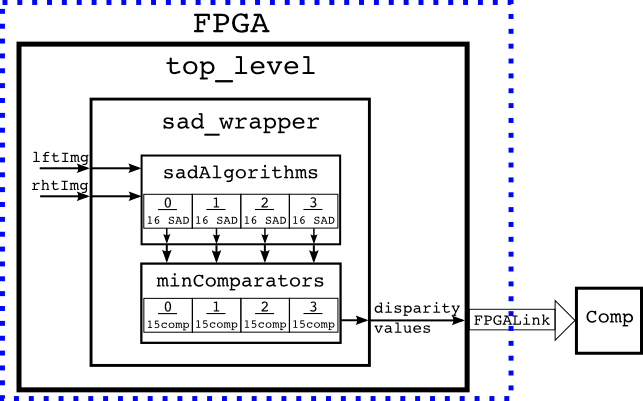
\includegraphics[width=150mm]{figures/top_level_rtl.png}
		\captionfonts
		\caption{The overview of the structure used for implementing the 9x9 window. The 7x7 window has two less SAD and minComp each.}
		\label{fig:topLevel_rtl}
	\end{center}
\end{figure}

\section{FPGALink}
\label{sec:fpgalink}

FPGALink~\cite{fpgalink} was used to facilitate communications between the computer (host) and the FPGA (Atlys board) over USB. An overview of how the FPGALink works between the host and FPGA is shown in Figure~\ref{fig:fpgalink}. The FPGALink has two possible communication modules to choose from, FX2 and EPP. According to~\cite{fpgalink}, FX2 has an observed throughput around 26 MB/s, while EEP has a observed throughput of around 1.26 MB/s. FX2 was used due to its higher throughput.

\begin{figure}[h]
	\begin{center}
		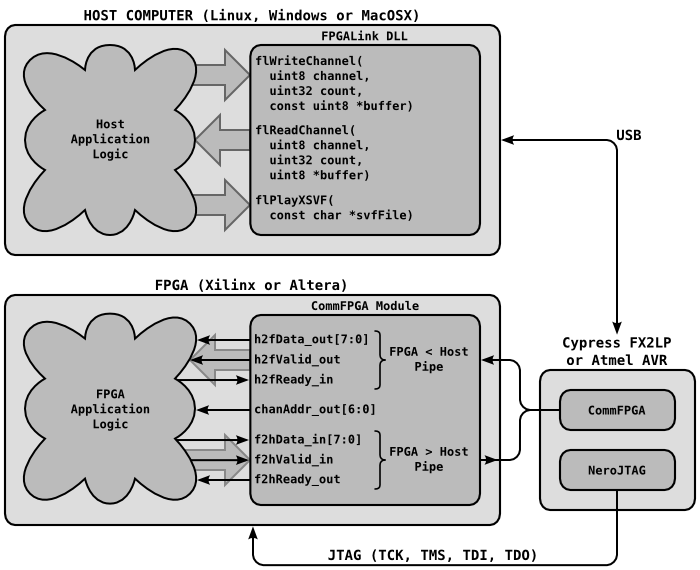
\includegraphics[width=150mm]{figures/fpgalinkOverview.png}
		\captionfonts
		\caption{Overview of FPGALink communications between host computer and FPGA~\cite{fpgalink}.}
		\label{fig:fpgalink}
	\end{center}
\end{figure}


\newcolumntype{+}{>{\global\let\currentrowstyle\relax}}
\newcolumntype{^}{>{\currentrowstyle}}
\newcommand{\rowstyle}[1]{\gdef\currentrowstyle{#1}%
#1\ignorespaces
}

\chapter{Experiments and Results}
\label{sec:exp}

The experiments and results presented in this section used the FPGA Atlys board and a desktop computer that has an i7 CPU 950 at 3.07 GHz, 16 GB of RAM, and runs Ubuntu 64-bit. Due to hardware and timing issues with the DDR RAM on the FPGA board, the board was unable to hold all of the data for both images. Part of the rows of both images were sent to the FPGA board from the computer. The board processed the data and send the disparity values back to the computer. The computer then provide the board with the next set of data and so on until the entire disparity map was created. This was used to test the quality and accuracy of the disparity maps from the FPGA implementation in comparison to computer implementations. The transfer time of sending both images to the FPGA board was not a real-time solution. To test for the maximum possible frames per second the SAD wrapper perform at, testbench simulations were used to obtain the time it should take to produce a disparity map on the board at a 100 MHz clock. The Atlys board has a 100 MHz clock on it, so that determined the clock cycle of 10 ns in the testbench simulations.

\section{Window Size Selection}
\label{sec:windowSize}

The size of the window (e.g. 9x9 pixels) affects the quality of the disparity map (see Figure~\ref{fig:tsukubaWinSize}) and the number of computations required to create the disparity map. The 3x3 window size in Figure~\ref{fig:tsukuba3x3} is processed the fastest out of the window sizes shown since each SAD calculation only has 9 pairs of pixels. The 13x13 window in Figure~\ref{fig:tsukuba13x13} has 169 pairs of pixels, which will require 160 more calculations per SAD value. However, the 13x13 window has the least amount of noise in its disparity map, but it loses some detail as shown by comparing the neck of the lamp in the foreground of the image compared to the lamp necks in the other images. Also, as the window size gets larger, more resources are needed on the FPGA board. The 7x7 and 9x9 window sizes were used because they provided a good compromise on the amount of noise in the disparity maps and the amount of hardware resources required for implementation. 

\begin{figure}
\begin{center}
	\begin{subfigure}{0.45\textwidth}
		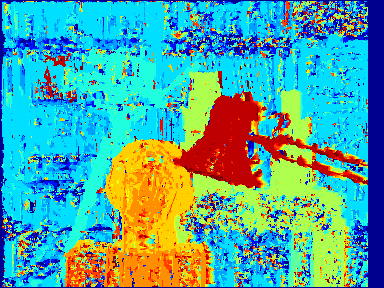
\includegraphics[width=\textwidth]{figures/sad_tsukuba_3x3_0-15.png}
		\caption{SAD 3x3 Window Disparity Map}
		\label{fig:tsukuba3x3}
	\end{subfigure}
	\begin{subfigure}{0.45\textwidth}
		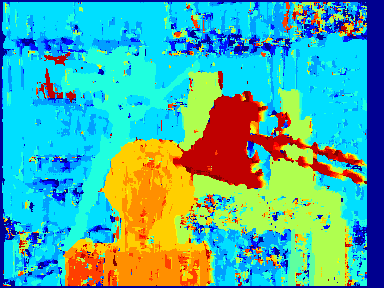
\includegraphics[width=\textwidth]{figures/sad_tsukuba_5x5_0-15.png}
		\caption{SAD 5x5 Window Disparity Map}
		\label{fig:tsukuba5x5}
	\end{subfigure}
	\\
	\begin{subfigure}{0.45\textwidth}
		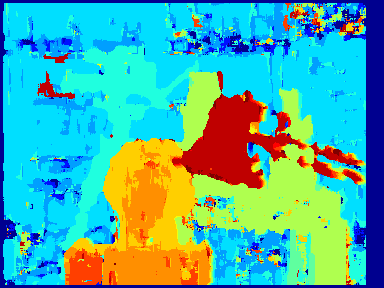
\includegraphics[width=\textwidth]{figures/sad_tsukuba_7x7_0-15.png}
		\caption{SAD 7x7 Window Disparity Map}
		\label{fig:tsukuba7x7}
	\end{subfigure}
	\begin{subfigure}{0.45\textwidth}
		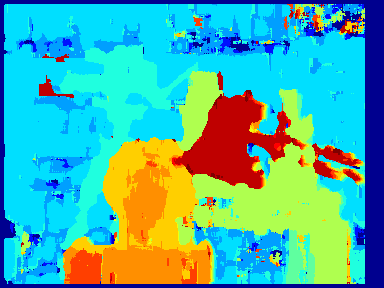
\includegraphics[width=\textwidth]{figures/sad_tsukuba_9x9_0-15.png}
		\caption{SAD 9x9 Window Disparity Map}
		\label{fig:tsukuba9x9}
	\end{subfigure}
	\\
	\begin{subfigure}{0.45\textwidth}
		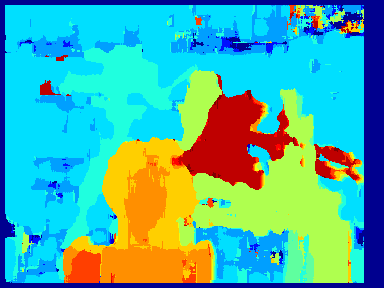
\includegraphics[width=\textwidth]{figures/sad_tsukuba_11x11_0-15.png}
		\caption{SAD 11x11 Window Disparity Map}
		\label{fig:tsukuba11x11}
	\end{subfigure}
	\begin{subfigure}{0.45\textwidth}
		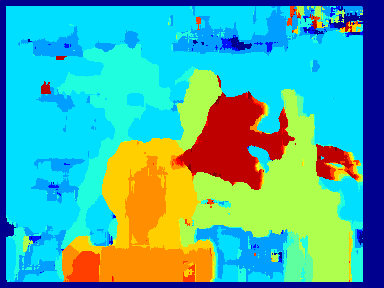
\includegraphics[width=\textwidth]{figures/sad_tsukuba_13x13_0-15.png}
		\caption{SAD 13x13 Window Disparity Map}
		\label{fig:tsukuba13x13}
	\end{subfigure}
	\captionfonts
	\caption{Window size comparisons for disparity maps~\cite{matlab} of the Tskukuba image pair~\cite{middlebury}.}
	\label{fig:tsukubaWinSize}
\end{center}
\end{figure}

\section{Resource Utilization on FPGA}
\label{sec:utilize}

See Table~\ref{table:utilize} for resource utilization. The 7x7 window implementation actually uses more resources on the FPGA board than the 9x9 window implementation due to the amount of parallel calculations used in the SAD algorithm. There is still plenty of space on the board for other top level entity designs for this SAD module.

\begin{table}
\begin{center}
	\begin{tabular}{| p{2cm} | p{2cm} | p{2.5cm} | p{3cm} | p{2.5cm} |}
		\hline
		\rowstyle{\bfseries} Window Size & 
		\rowstyle{\bfseries} \# of pixels in parallel & 
		\rowstyle{\bfseries} \# of Slice Registers, out of 54,576 &
		\rowstyle{\bfseries} \# of Slice LUTs, out of 27,288 & 
		\rowstyle{\bfseries} \# of occupied Slices, out of 6,822 %& 
		%\rowstyle{\bfseries} \# of MUXCYs, out of 13,644
		\tabularnewline
		\hline
		7x7 & 2 & 8,465 (15\%) & 17,220 (63\%) & 5,640 (82\%) %&  3,796 (27\%)
		\tabularnewline
		\hline 
		9x9 & 4 & 8,136 (14\%) & 16,038 (58\%) & 4,719 (69\%) %&  2,280 (16\%)
		\tabularnewline
		\hline 
	\end{tabular}
	\captionfonts
	\caption{Resource utilization on the FPGA Atlys board for both window implementations.}
	\label{table:utilize}
\end{center}
\end{table}

\section{Testbench Simulation}
\label{sec:testbench}

See Figure~\ref{fig:tb_9x9} and Figure~\ref{fig:tb_7x7} in Appendix~\ref{sec:appdxD} for the testbench simulations for the 9x9 window and 7x7 window implementations, respectively.

The signal h2fvalid\_i, near the top of the figures, went high when image data is sent to the SAD wrapper. The first time h2fvalid\_i went high until the second time it went high was when the initial rows were given to the wrapper up to when the initial disparity values were produced. A cycle began afterwards where h2fvalid\_i would go high for several clock cycles and then go low for several more clock cycles. The high section represented when the next row was sent to the wrapper while the low section represented the time it took to calculate the SAD values and produce the next disparity values. The wrapper has been designed to allow both the template image data and the search image data to be sent to the wrapper at the same time, thus reducing the amount of time taken to get all necessary data into the wrapper. When the signal f2hready\_i goes high, it means that the disparity values are being sent out of the wrapper.

\subsection{9x9 Window Implementation Runtime}
\label{sec:testbench9x9}

Based on the testbench simulation in Fig.~\ref{fig:tb_9x9} the theoretical frames per second can be inferred for different image sizes. The simulation assumes the 100 MHz clock on the FPGA is used, which is the clock frequency used on the Atlys board. The clock cycle duration is therefore 10 ns long.

In the testbench simulation, the window size is 9x9 and 4 pixels are processed in parallel. The first section of the simulation includes the initial image data given to the SAD wrapper up to the point where that data's disparity values are returned. This section takes 3.35 us. After that, a constant cycle is produced, which includes the SAD wrapper taking in the next row and producing the next disparity values. This cycle takes 1.22 us. A 640x480 image has 307,200 pixels, which will produce a disparity map of 617x472, or 291,224 pixels. Disparity values are not produced for pixels where either the window would run off the image or where there is not enough room for the 16 SAD values to be calculated for the pixel. Since 4 pixels are processed in parallel, 291,224 pixels are divided by 4 pixels/iteration, giving 72,806 iterations. So, 72,805 iterations times 1.22 us/iteration plus 3.35 us (initial section, hence minus one on number of iterations) gives 88,826.67 us or approximately 0.0888 seconds per frame. Therefore, an image size of 640x480 can be processed at around 11.26 frames per second. Table~\ref{table:tb_9x9} shows the theoretical frame rate for the image sizes used in this chapter.

\begin{table}
	\begin{center}
		\begin{tabular}{|c|c|c|c|c|}
			\hline 
				\rowstyle{\bfseries} Image & 
				\rowstyle{\bfseries} Image Width & 
				\rowstyle{\bfseries} Image Height & 
				\rowstyle{\bfseries} Sec/frame & 
				\rowstyle{\bfseries} Frames/sec
			\tabularnewline
			\hline 
			VmodCAM & 640 & 480 & 0.0888 & 11.26
			\tabularnewline
			\hline 
			Tsukuba & 384 & 288 & 0.0308 & 32.43
			\tabularnewline
			\hline 
			Venus & 434 & 383 & 0.0470 & 21.27
			\tabularnewline
			\hline 			
			\end{tabular}
		\captionfonts
		\caption{9x9 window for theoretical runtime for the FPGA board for different image sizes.}
		\label{table:tb_9x9}
	\end{center}
\end{table}

\subsection{7x7 Window Implementation Runtime}
\label{sec:testbench7x7}

Based on the testbench simulation in Fig.~\ref{fig:tb_7x7} the theoretical frame rate can be inferred for different image sizes. The simulation uses a clock cycle of 10 ns.

In the testbench simulation, the window size is 7x7 and 2 pixels are processed in parallel. The first section of the simulation includes the initial image data given to the SAD wrapper up to the point where that data's disparity values are returned. This section takes 1.78 us. After that, a constant cycle is produced allowing the SAD wrapper to get the next row and produce the next disparity values, which takes 0.42 us. A 640x480 image has 307,200 pixels, which will produce a disparity map of 619x474, which is 293,406 pixels. Disparity values are not produced for pixels that either the windows cannot fit on or there is not enough room for the 16 SAD values to be calculated for the pixel. Since 2 pixels are processed in parallel, 293,406 pixels is divided by 2 pixels/iteration, giving 146,703 iterations. So, 146,702 iterations times 0.42 us/iteration plus 1.78 us (initial section, hence minus one on number of iterations) gives 61,617.04 us or approximately 0.0616 seconds per frame. Therefore, an image size of 640x480 can be processed at around 16.23 frames per second. Table~\ref{table:tb_7x7} shows the theoretical frame rate for the image sizes used in this chapter.


\begin{table}
	\begin{center}
		\begin{tabular}{|c|c|c|c|c|}
			\hline
				\rowstyle{\bfseries} Image & 
				\rowstyle{\bfseries} Image Width & 
				\rowstyle{\bfseries} Image Height & 
				\rowstyle{\bfseries} Sec/frame & 
				\rowstyle{\bfseries} Frames/sec
			\\ \hline 
			VmodCAM & 640 & 480 & 0.0616 & 16.23
			\\ \hline 
			Tsukuba & 384 & 288 & 0.0215 & 46.51
			\\ \hline 
			Venus & 434 & 383 & 0.0327 & 30.58
			\\ \hline 
		\end{tabular}	
		\captionfonts
		\caption{7x7 window for theoretical runtime for the FPGA board for different image sizes.}
		\label{table:tb_7x7}
	\end{center}
\end{table}

\section{Test Image Pairs}
\label{sec:runtime}

In this section, FPGA disparity maps are compared to disparity maps created using Python. Part of the SAD algorithm implementation in Python is shown in Appendix~\ref{sec:appdxE}. The Python SAD version is performed completely in serial, so 1 pixel at a time. The images the Python version produced are used to compare disparity map quality and runtime of the algorithm.

\subsection{Data Overflows}
\label{sec:overflow}

The code for the hardware to be generated is designed in VHDL. The size of the data used for storing logic and values in hardware is defined during the coding process. In the SAD algorithm, it is possible for the SAD value to become much larger than the individual pixel values. For example, the pixel values range from 0 to 255, or 8 bits, while some SAD values could be over 4,095 and need to be stored in more than 12 bits. Most SAD values were under 4,096, so to account for those that were above it, the SAD algorithm use 14 bits to account for any values from 0 to 16,383. Figure~\ref{fig:overflow} shows what can happen when the data size allotted for the SAD algorithm is not large enough (i.e. only having 10 bits for storage). The data used is unsigned, so when it goes above the highest supported value, it goes back to 0 and continues from there.

Since most of the values were below 4,096, a measure was put in place in order to reduce the amount of bits needed during the minimum comparisons. If a SAD value was greater than 4,095, then 4,095 was returned for the calculated SAD because the greater the value, the less likely that search pixel is the correct corresponding one to the template pixel. In Figure~\ref{fig:tsukubaDispMap} and Figure~\ref{fig:venusDispMap}, the only noticeable difference in the Python to FPGA comparisons is at the top of the images. The colors, warmer is closer and cooler is farther away, show that the top areas are thought to be closer than they actually are in the FPGA images. For a robot, it would be better to error on the side of thinking an object is closer than it actually is because the robot will be less prone to collide with the object. If a robot thought an object was farther away than it actually was, then the likelihood of collision would increase.

\begin{figure}[h]
	\begin{center}
		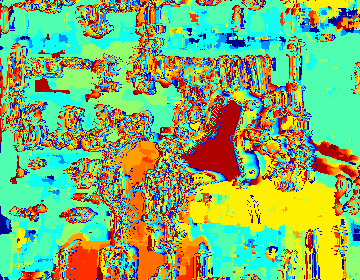
\includegraphics[width=80mm]{figures/tsukuba_disp9x9_2_sad_overflow.png}
		\captionfonts
		\caption{Data overflow for Tskukuba image pair~\cite{middlebury}.}
		\label{fig:overflow}
	\end{center}
\end{figure}

\subsection{Tsukuba}
\label{sec:tsukuba}

In Figure~\ref{fig:tsukubaL} and Figure~\ref{fig:tsukubaR}, the Tsukuba image pair is shown. Figure~\ref{fig:tsukubaDispMap} shows how the 7x7 window implementation is slightly noisier than the 9x9 window implementation. As discussed in Section~\ref{sec:overflow}, the only noticeable difference between the Python implementation and the FPGA implementation is at the top of the disparity maps. This difference is caused by not having enough similarities between corresponding regions. It is possible for certain parts of an object in one image to be occluded in the image. This causes SAD values to be greater than normal. 

For Tsukuba, the FPGA version has a theoretical runtime of 32.43 and 46.51 frames per second for the 9x9 and 7x7 window implementations, respectively, from Table~\ref{table:tb_9x9} and Table~\ref{table:tb_7x7}. The serial Python implementation took 7.81 minutes for a 9x9 window with a disparity range of 16. The 7x7 window implementation with a disparity range of 16 in Python took 4.22 minutes to complete.

\begin{figure}
\begin{center}
	\begin{subfigure}{0.45\textwidth}
		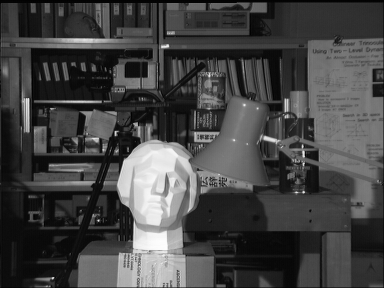
\includegraphics[width=\textwidth]{figures/tsukubaL.jpg}
		\caption{Left Tsukuba Grayscale Image}
		\label{fig:tsukubaL}
	\end{subfigure}
	\begin{subfigure}{0.45\textwidth}
		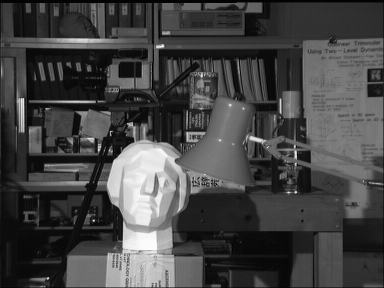
\includegraphics[width=\textwidth]{figures/tsukubaR.jpg}
		\caption{Right Tsukuba Grayscale Image}
		\label{fig:tsukubaR}
	\end{subfigure}
	\\
	\begin{subfigure}{0.45\textwidth}
		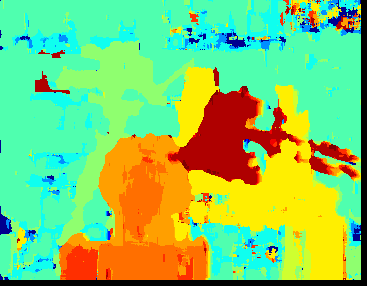
\includegraphics[width=\textwidth]{figures/tsukuba_9x9_python3.png}
		\caption{Python 9x9 Disparity Map}
		\label{fig:tsukubaPy}
	\end{subfigure}
	\begin{subfigure}{0.45\textwidth}
		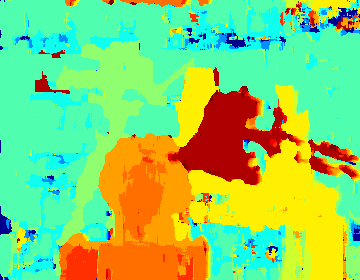
\includegraphics[width=\textwidth]{figures/tsukuba_9x9_fpga.png}
		\caption{FPGA 9x9 Disparity Map}
		\label{fig:tsukubaFPGA}
	\end{subfigure}
	\\
	\begin{subfigure}{0.45\textwidth}
		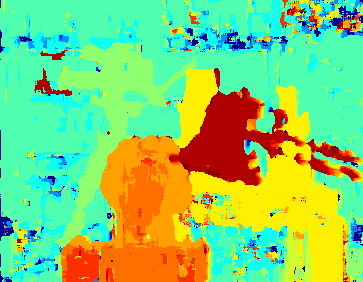
\includegraphics[width=\textwidth]{figures/tsukuba_7x7_python3.png}
		\caption{Python 7x7 Disparity Map}
		\label{fig:tsukubaPy}
	\end{subfigure}
	\begin{subfigure}{0.45\textwidth}
		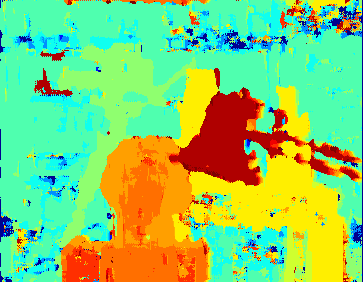
\includegraphics[width=\textwidth]{figures/tsukuba_7x7_fpga.png}
		\caption{FPGA 7x7 Disparity Map}
		\label{fig:tsukubaFPGA}
	\end{subfigure}
	\captionfonts
	\caption{Disparity map comparison of the Tskukuba image pair~\cite{middlebury}.}
	\label{fig:tsukubaDispMap}
\end{center}
\end{figure}

\subsection{Venus}
\label{sec:venus}

In Figure~\ref{fig:venusL} and Figure~\ref{fig:venusR}, the Venus image pair is shown. In the image pair, the newspaper articles are flat and slanted, relative to the cameras. This gradual slope, also present in the background, can be difficult for the SAD algorithm to deal with; however, the algorithm is still able to give a fairly accurate representation of the depth in the image. It also causes the gradient pattern shown in the disparity maps. The 7x7 window depth maps have more noise than the 9x9 window depth maps.

For Venus, the FPGA version has a theoretical runtime of 21.27 and 30.58 frames per second for the 9x9 and 7x7 window implementations, respectively, from Tbl.~\ref{table:tb_9x9} and Tbl.~\ref{table:tb_7x7}. The serial Python implementation took 8.15 minutes for a 9x9 window with a disparity range of 16. The 7x7 window implementation with a disparity range of 16 in Python took 5.00 minutes to complete.

\begin{figure}
\begin{center}
	\begin{subfigure}{0.45\textwidth}
		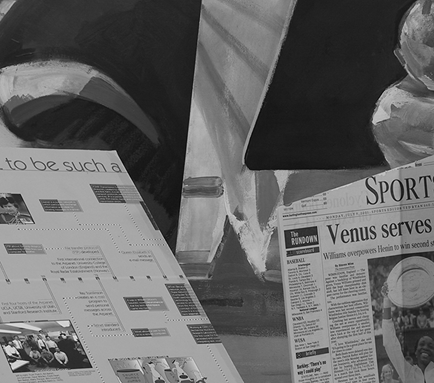
\includegraphics[width=\textwidth]{figures/venusL.png}
		\caption{Left Venus Grayscale Image}
		\label{fig:venusL}
	\end{subfigure}
	\begin{subfigure}{0.45\textwidth}
		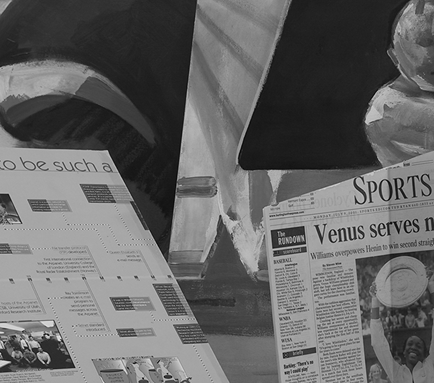
\includegraphics[width=\textwidth]{figures/venusR.png}
		\caption{Right Venus Grayscale Image}
		\label{fig:venusR}
	\end{subfigure}
	\\
	\begin{subfigure}{0.45\textwidth}
		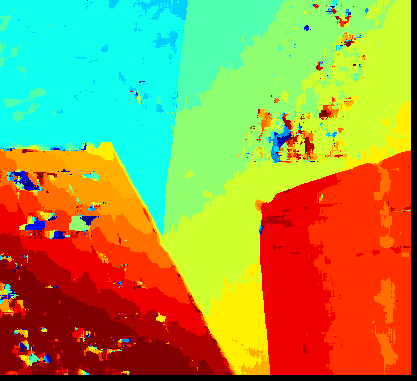
\includegraphics[width=\textwidth]{figures/venus_9x9_python3.png}
		\caption{Python 9x9 Disparity Map}
		\label{fig:venusPy}
	\end{subfigure}
	\begin{subfigure}{0.45\textwidth}
		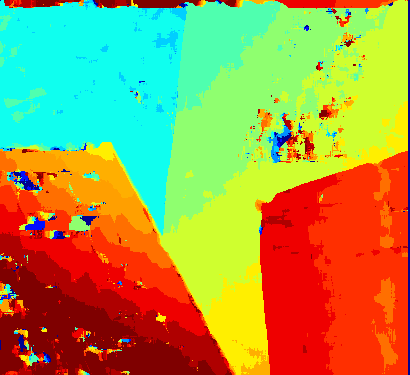
\includegraphics[width=\textwidth]{figures/venus_9x9_fpga.png}
		\caption{FPGA 9x9 Disparity Map}
		\label{fig:venusFPGA}
	\end{subfigure}
	\\
	\begin{subfigure}{0.45\textwidth}
		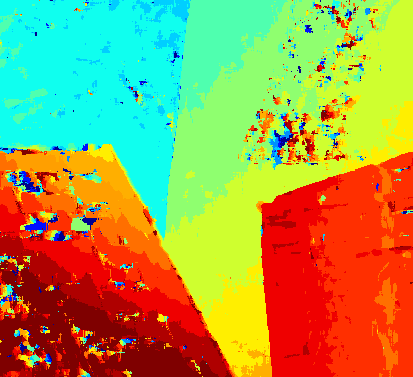
\includegraphics[width=\textwidth]{figures/venus_7x7_python3.png}
		\caption{Python 7x7 Disparity Map}
		\label{fig:venusPy}
	\end{subfigure}
	\begin{subfigure}{0.45\textwidth}
		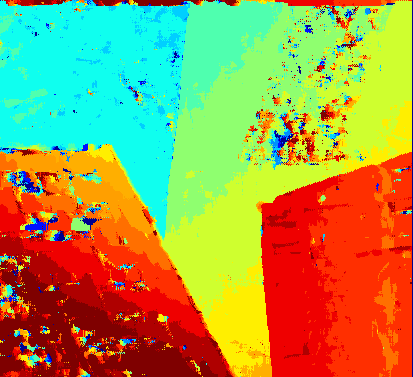
\includegraphics[width=\textwidth]{figures/venus_7x7_fpga.png}
		\caption{FPGA 7x7 Disparity Map}
		\label{fig:venusFPGA}
	\end{subfigure}
	\captionfonts
	\caption{Disparity map comparison of the Venus image pair~\cite{middlebury}.}
	\label{fig:venusDispMap}
\end{center}
\end{figure}


\subsection{Cones}
\label{sec:cones}

In Figure~\ref{fig:conesL} and Figure~\ref{fig:conesR}, the Venus image pair is shown. Figure~\ref{fig:conesDispMap} shows the issue of objects in an image pair being too close to the stereo cameras. The closer an object is to the stereo cameras, the greater its disparity value will be. Using the SAD algorithm with a 9x9 window and a disparity range of 60 (as opposed to the range of 16 used on the FPGA board) produces the results in Figure~\ref{fig:conesMatlab}. When the disparity range is not high enough, the disparity map in Figure~\ref{fig:conesPy} is produced.

\begin{figure}
\begin{center}
	\begin{subfigure}{0.45\textwidth}
		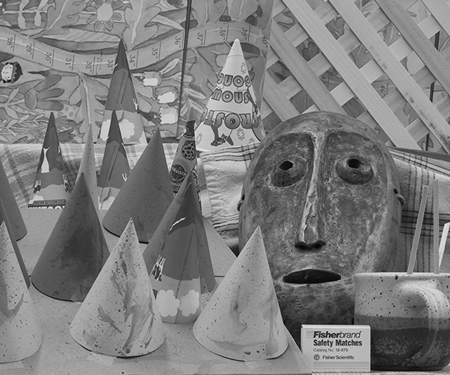
\includegraphics[width=\textwidth]{figures/conesL.png}
		\caption{Left Cones Grayscale Image}
		\label{fig:conesL}
	\end{subfigure}
	\begin{subfigure}{0.45\textwidth}
		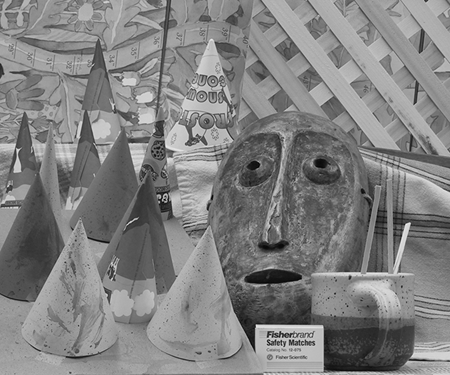
\includegraphics[width=\textwidth]{figures/conesR.png}
		\caption{Right Cones Grayscale Image}
		\label{fig:conesR}
	\end{subfigure}
	\\
	\begin{subfigure}{0.45\textwidth}
		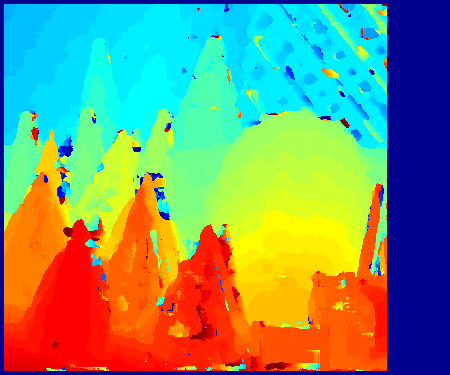
\includegraphics[width=\textwidth]{figures/cones_9x9_matlab_0-59.png}
		\caption{9x9 at Disparity Range of 60 ~\cite{matlab}}
		\label{fig:conesMatlab}
	\end{subfigure}
	\begin{subfigure}{0.45\textwidth}
		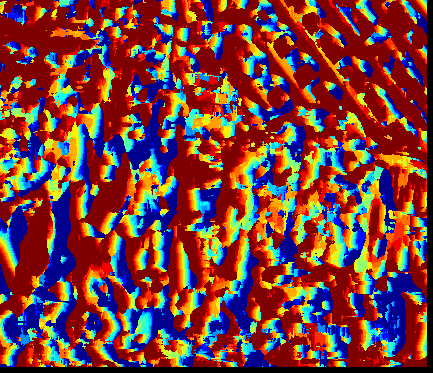
\includegraphics[width=\textwidth]{figures/cones_9x9_python3.png}
		\caption{9x9 at Disparity Range of 16}
		\label{fig:conesPy}
	\end{subfigure}
	\captionfonts
	\caption{Disparity map comparison of the Cones image pair ~\cite{middlebury}.}
	\label{fig:conesDispMap}
\end{center}
\end{figure}






\chapter{Conclusions}
Concluded.

In the Future!

% ------------- End main chapters ----------------------

\clearpage
\bibliographystyle{plain}
\bibliography{references}

%\begin{appendix}
%%\addcontentsline{toc}{chapter}{\appendixnamelower}
%\include{Appendix}
%\end{appendix}

\end{document}